% Koko
\documentclass[blue,normal,cn]{elegantnote}
\usepackage{array}
\usepackage{courier}
\usepackage{xcolor}
\usepackage{tabulary}
\definecolor{light-gray}{gray}{0.95}
\newcommand{\code}[1]{\colorbox{light-gray}{\texttt{#1}}}
\newfontfamily\courier{Courier New}
\lstset{linewidth=1.1\textwidth,
	numbers=left,
	basicstyle=\small\courier,
	numberstyle=\tiny\courier,
	keywordstyle=\color{blue}\courier,
	commentstyle=\it\color[cmyk]{1,0,1,0}\courier, 
	stringstyle=\it\color[RGB]{128,0,0}\courier,
	frame=single,
	backgroundcolor=\color[RGB]{245,245,244},
	breaklines,
	extendedchars=false, 
	xleftmargin=2em,xrightmargin=2em, aboveskip=1em,
	tabsize=4, 
	showspaces=false
	basicstyle=\small\courier
}
\title{用户需求说明书}
\version{1.0.1}
\date{\today}

\begin{document}
\author{
	\begin{tabular}[t]{c}
		2017211305 班 E 组 \\
		于海鑫\ 徐翔\ 赵泉斌\ 郭朝宇\ 郭璐
	\end{tabular}
}
\maketitle

\tableofcontents

\section{文档介绍}

\subsection{文档目的}
\begin{enumerate}
	\item 详细地描述分布式温控系统的设计及开发流程
	\item 作为软件开发者的参考与知道,方便软件的开发,迭代以及维护
\end{enumerate}

\subsection{文档范围}
我们的文档围绕分布式温控系统展开,记录该系统的性能、功能以及运行方式,全面介绍软件的架构,分析用户的需求。

\subsection{读者对象}
\begin{enumerate}
	\item 酒店管理方、使用方
	\item 软件开发设计方
\end{enumerate}

\subsection{参考文献}

\begin{itemize}
	\item 《\emph{软件工程模型与方法}》 肖丁等\ 北京邮电大学出版社
	\item 《\emph{美的空调使用说明书}》
\end{itemize}

\section{产品介绍}

\subsection{产品的功能及作用}
自助计费分布式中央温控系统(以下简称“分布式温控计费系统”或“本系统” )为适用于酒店等环境的空调计费系统。其使用自助计费的方式,使得入住的客户可以根据个人的需求设置合适的温度,同时可以通过房间内部提供的显示屏或者微信小程序等方式查看当前空调状态、付费金额以及收费标准等信息。酒店方则可以实时监控各个空调的状态、获取空调的使用详单以及统计报表等信息,也可以通过网页查看/管理用户信息,方便在客户退房时进行结账操作。

\subsection{系统面向的用户群体}

\subsubsection{客户}
本系统的直接客户为快捷廉价酒店,其主要诉求为:以较低的成本获取到高性能的产品,以 ”廉价、实用、个性化、智能化“ 为噱头吸引客户。以此保证自身的利润,同时响应国家的节能绿色环保理念。

\subsubsection{终端用户}
本系统的终端用户为选择快捷廉价酒店住宿的人员,其诉求为获取廉价优质的服务。

\subsubsection{产品应当遵循的标准或规范}

\begin{itemize}
	\item \textbf{GB50736-2012}\ 《\emph{民用建筑供暖通风与空气调节设计规范}》
	\item \textbf{JGJ26-95}\ 《\emph{民用建筑节能设计标准(采暖居住建筑部分)}》
	\item \textbf{JGJ62-2014}\ 《\emph{旅馆建筑设计规范}》
\end{itemize}

\section{功能性需求}

\subsection{主控端}

\subsubsection{控制模块}
这一模块的作用为处理来自客户端的请求、向客户端发送指令以调节空调的运行。

\begin{center}
	\begin{tabular}{|>{\centering}m{0.15\textwidth}|m{0.7\textwidth}|}
		\hline
		\textbf{功能名称} & \multicolumn{1}{c|}{\textbf{描述}}                           \\
		\hline
		数据收集          & 从各个客户端中收集数据,同时监控中央空调的状态               \\
		\hline
		数据保存          & 将采集到的信息存储到数据库中                                 \\
		\hline
		空调控制          & 根据收集到的数据,结合各个用户的需求,调控中央空调的运行状态 \\
		\hline
		从控控制          & 根据各个用户的不同需求,控制各个从控端的空调状态             \\
		\hline
		异常报警          & 当中央空调或是某一从控端出现异常时,及时通知系统的维护人员   \\
		\hline
	\end{tabular}
\end{center}

\subsubsection{计费模块}
这一模块的作用为使用设置好的计费标准,依照控制模块收集到的数据计算各个用户的付费金额。

\begin{center}
	\begin{tabular}{|>{\centering}m{0.15\textwidth}|m{0.7\textwidth}|}
		\hline
		\textbf{功能名称} & \multicolumn{1}{c|}{\textbf{描述}}                                 \\
		\hline
		计费设置          & 设置计费标准,实际实现时会表示为几个特定的参数                     \\
		\hline
		费用计算          & 处理来自控制模块的数据,通过设置好的计费标准计算用户的付费金额     \\
		\hline
		支付功能          & 向用户发送详细的计费信息,同时支持用户使用二维码支付或者到前台付费 \\
		\hline
	\end{tabular}
\end{center}

\subsubsection{管理模块}
这一模块的作用为为酒店管理方提供一个修改用户信息、监控空调等操作的控制台。

\begin{center}
	\begin{tabular}{|>{\centering}m{0.15\textwidth}|m{0.7\textwidth}|}
		\hline
		\textbf{功能名称} & \multicolumn{1}{c|}{\textbf{描述}}                                \\
		\hline
		账户管理          & 提供用户绑定、权限设置、身份验证等功能                            \\
		\hline
		实时监控          & 实时地显示各个空调的运行情况、各个房间的付费金额等信息            \\
		\hline
		报表导出          & 可以将系统的能耗、收益等统计信息导出为 \code{xlsx} 等格式以供分析 \\
		\hline
	\end{tabular}
\end{center}

\subsection{从控端}

\subsubsection{支付模块}

\begin{center}
	\begin{tabular}{|>{\centering}m{0.15\textwidth}|m{0.7\textwidth}|}
		\hline
		\textbf{功能名称} & \multicolumn{1}{c|}{\textbf{描述}}                     \\
		\hline
		费用显示          & 在用户使用空调时,显示当前的费用以及收费标准           \\
		\hline
		支付提示          & 在用户退房或者主动要求支付时,弹出二维码以提示用户支付 \\
		\hline
		节能警示          & 在用户的功率过大时,提示用户节能环保,降低功率         \\
		\hline
	\end{tabular}
\end{center}

\subsubsection{管理模块}

\begin{center}
	\begin{tabular}{|>{\centering}m{0.15\textwidth}|m{0.7\textwidth}|}
		\hline
		\textbf{功能名称} & \multicolumn{1}{c|}{\textbf{描述}}                                   \\
		\hline
		状态显示          & 在用户使用时,显示当前房间的状态                                     \\
		\hline
		模式调节          & 调节空调的模式,包含 制冷 制热 送风 干燥 辅热 定时 换气 睡眠 扫风 等 \\
		\hline
		风速调节          & 可以将风速调节为 自动、低速、中速、高速三个档次                      \\
		\hline
		温度调节          & 除去送风模式外均可调节温度,调节范围为 16-30°C                       \\
		\hline
		空调电源          & 按动电源键以打开或者关闭空调,用户离开房间时自动关闭空调             \\
		\hline
	\end{tabular}
\end{center}

\section{非功能性需求}

\subsection{主控端}
我们的主控端应该满足如下需求:



\begin{center}
	\begin{tabular}{|>{\centering}m{0.15\textwidth}|m{0.7\textwidth}|}
		\hline
		\textbf{功能名称} & \multicolumn{1}{c|}{\textbf{描述}}                                                                                                                                                                                                         \\
		\hline
		用户友好          & 主控机界面应简洁美观,实用性强;各个按钮在界面中合理分布,方便管理员管理、监控。主控机应该能够清楚、简洁地显示各个从控机的状态,各机器的能耗统计数据及费用报表                                                                             \\
		\hline
		安全性            & 主控机应提供管理员身份认证、授权控制、以及系统安全性等方面的保证。同时能够监控系统内部的流量情况,发现异常流量情况时及时发出警告。对系统外部及内部的潜在攻击有一定的防御能力                                                               \\
		\hline
		鲁棒性            & 主控机应具有应对可能的并发大规模请求的能力,保证系统不会在大量用户的同时请求下崩溃                                                                                                                                                         \\
		\hline
		易用性            & 主控机的使用应尽可能地保持简单,并且对主控机的使用应该提供尽可能详细的使用说明及培训资料,保证管理员能够尽可能简单、快捷地使用主控机                                                                                                       \\
		\hline
		可靠性            & 系统需要全天候运行,并且要求能快速部署,特别是在系统出现故障时,能够快速告知管理员,并能够提供应急服务,保证酒店的正常工作不受影响                                                                                                         \\
		\hline
		可维护性          & 主控机系统应保证良好的可维护性。主控机应保证定时或在事件驱动下输出日志,以供维护人员可以监控和观察系统状态,在故障发生时及时的监测、诊断以及修复系统                                                                                       \\
		\hline
		可配置性          & 主控机的参数应该是可配置的,以使其可以通过不同的配置文件灵活部署于不同的平台及系统                                                                                                                                                         \\
		\hline
		可移植性          & 系统应能够在不同平台及操作系统下使用,具有良好的兼容性。在少量修改或者不作修改的基础上就可以方便、快捷地部署在不同的硬件及软件平台上                                                                                                       \\
		\hline
		可扩展性          & 分布式温控系统应具有对技术和业务需求变化的支持能力。当技术变化或业务变化时,不可避免将带来系统的改变。所以系统不仅可能面临进行设计实现的修改,甚至面临着进行产品定义的修改。因此,系统的设计应在系统架构上考虑能以尽量少的代价适应这种变化 \\
		\hline
	\end{tabular}
\end{center}

\subsection{从控端}
我们的从控端应该满足如下需求:

\begin{center}
	\begin{tabular}{|>{\centering}m{0.15\textwidth}|m{0.7\textwidth}|}
		\hline
		\textbf{功能名称} & \multicolumn{1}{c|}{\textbf{描述}}                                                                                                                                                                         \\
		\hline
		用户友好          & 从控机界面亦应简洁美观,实用性强;各个按钮在界面中合理分布,方便入住用户查看并操作。                                                                                                                       \\
		\hline
		安全性            & 从控机应提供住客及客房打扫人员等的身份认证及控制授权,保证从机不会被非法控制                                                                                                                               \\
		\hline
		鲁棒性            & 从控机在面对住客非正常使用时(如在短时间内多次按下模式切换键)能够正常地响应用户,保证系统不会崩溃                                                                                                           \\
		\hline
		易用性            & 从控机的界面应该清晰、简单,对新用户有足够的引导及帮助,保证用户能够正确地使用从控机发出温控请求                                                                                                           \\
		\hline
		可靠性            & 从控机应能保证较低的故障率,并且在故障发生时能够及时地告知主控机及工作人员进行故障修复                                                                                                                     \\
		\hline
		可维护性          & 从控机应该能够记录每一条发出的请求及来自主控机的控制命令,允许在管理员的操控下输出运行日志,记录系统运行状态。当发生故障时,保证维护人员可以监控和观察主、从控机状态,在故障发生时准确定位故障原因进行修复 \\
		\hline
		可配置性          & 从控机的参数应该是可配置的,以使得从控机通过不同的配置文件适应不同客户的需求。从控机系统可以记录不同用户的使用习惯,使得用户再次入住时不需要重复设置                                                       \\
		\hline
		可移植性          & 从控机软件应该能够方便快捷地部署在不同的平台上。如手机、壁挂面板等,以使得用户可以更方便地操控从控机                                                                                                       \\
		\hline
		可扩展性          & 在面对技术及需求不断的更新时,从控机应该能够方便快捷地进行升级扩展。这要求从控机与主控机架构上解耦,从软硬件两方面能够以尽可能小的成本升级修改                                                             \\
		\hline
	\end{tabular}
\end{center}

\section{其他需求}

\begin{itemize}
	\item \textbf{智能化}\ 电器的智能化是目前的大趋势,也是国家大力推进的技术革新。我们的空调从控端应该顺应潮流,增加与手机端的交互,甚至增加语音用纸等特性。
	\item \textbf{节能化}\ 我们的从控端应该通过一些算法,在不大幅度影响用户体验的情况下,减少空调的能耗。
	\item \textbf{低成本}\ 作为廉价酒店,我们的系统成本不应过高。
\end{itemize}

\section{领域模型}

\subsection{用户活动图}

详见 \textbf{图~\ref{fig:user}~}。

\begin{figure}[!htbp]
	\centering
	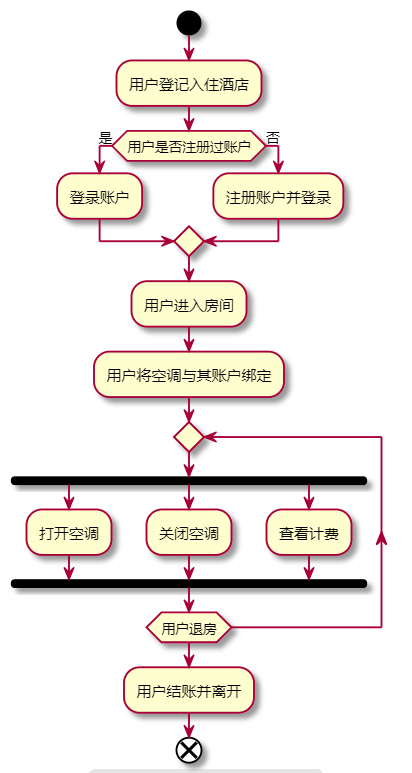
\includegraphics[width=.5\textwidth]{user}
	\caption{用户活动图}
	\label{fig:user}
\end{figure}

\subsection{概念模型}
详见 \textbf{图~\ref{fig:domain}~}。

\begin{figure}[!htbp]
	\centering
	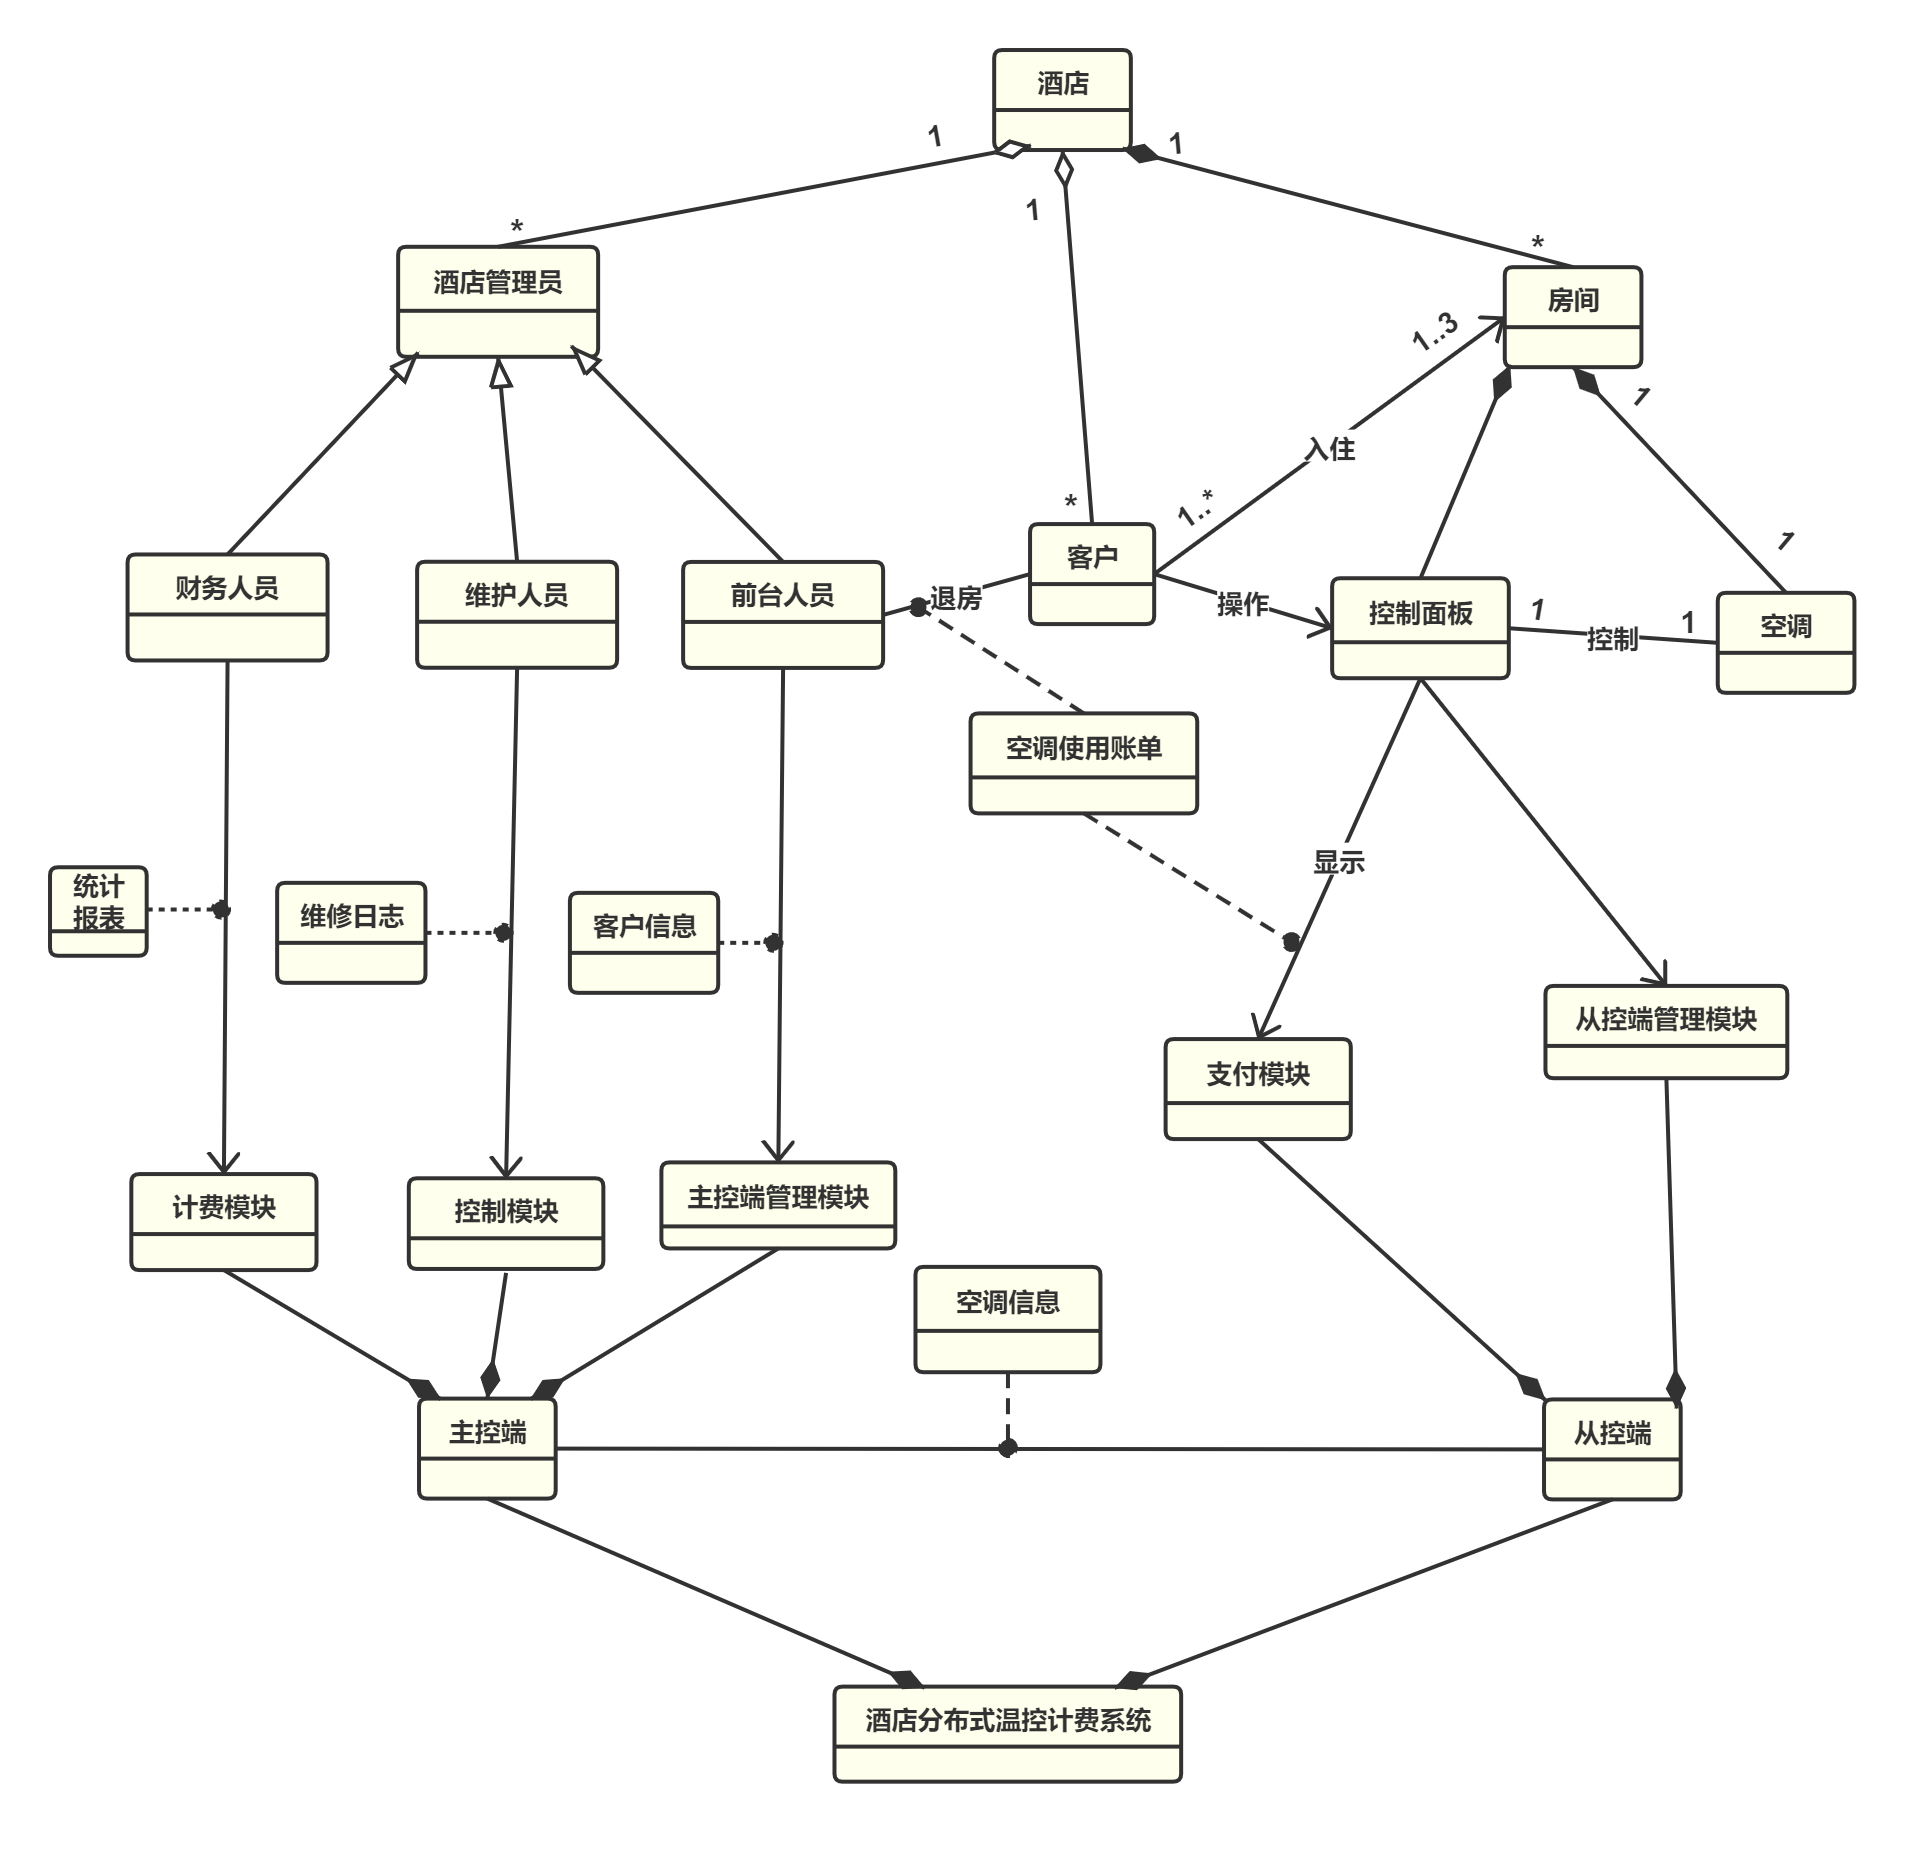
\includegraphics[width=1\textwidth]{domain}
	\caption{领域模型}
	\label{fig:domain}
\end{figure}

\end{document}